% =====================================================================
\clearpage
\partieENO{Le bilan}

Cette dernière partie fait le point sur le projet. Je commence par le montage réalisé le 12 novembre 2026 à l'UPF, avec des photos de la tour et de l'installation solaire. Je présente ensuite le tableau d'avancement de chaque fonction, avec ce qui est calculé, ce qui est vérifié sur du vrai matériel et ce qui reste à faire. Je liste ensuite les points ouverts, c'est-à-dire les hypothèses à remplacer par des mesures. Je termine par les prochaines étapes.

\subsection{Le montage réalisé à l'UPF}

Le 12 novembre 2026, nous avons monté la tour à l'UPF, mon coéquipier Gabriel Piritua et moi, ensemble. Le montage de l'installation est le fruit du travail de Gabriel : c'est lui qui a conçu et réalisé la structure métallique qui porte le panneau solaire et le plateau de l'armoire électrique. Nous avons monté ensemble le panneau solaire et la batterie sur cette structure, puis installé la tour sur son bac, devant elle, sur la coursive extérieure du bâtiment. Le régulateur solaire est en place dans l'armoire et son écran est allumé. Avant de brancher le panneau, il indiquait \qty{13,2}{V}, la tension de la batterie seule. Une fois le panneau branché, cette tension a monté avec l'ensoleillement, ce qui montre que le panneau charge bien la batterie.

\begin{figure}[H]
\centering
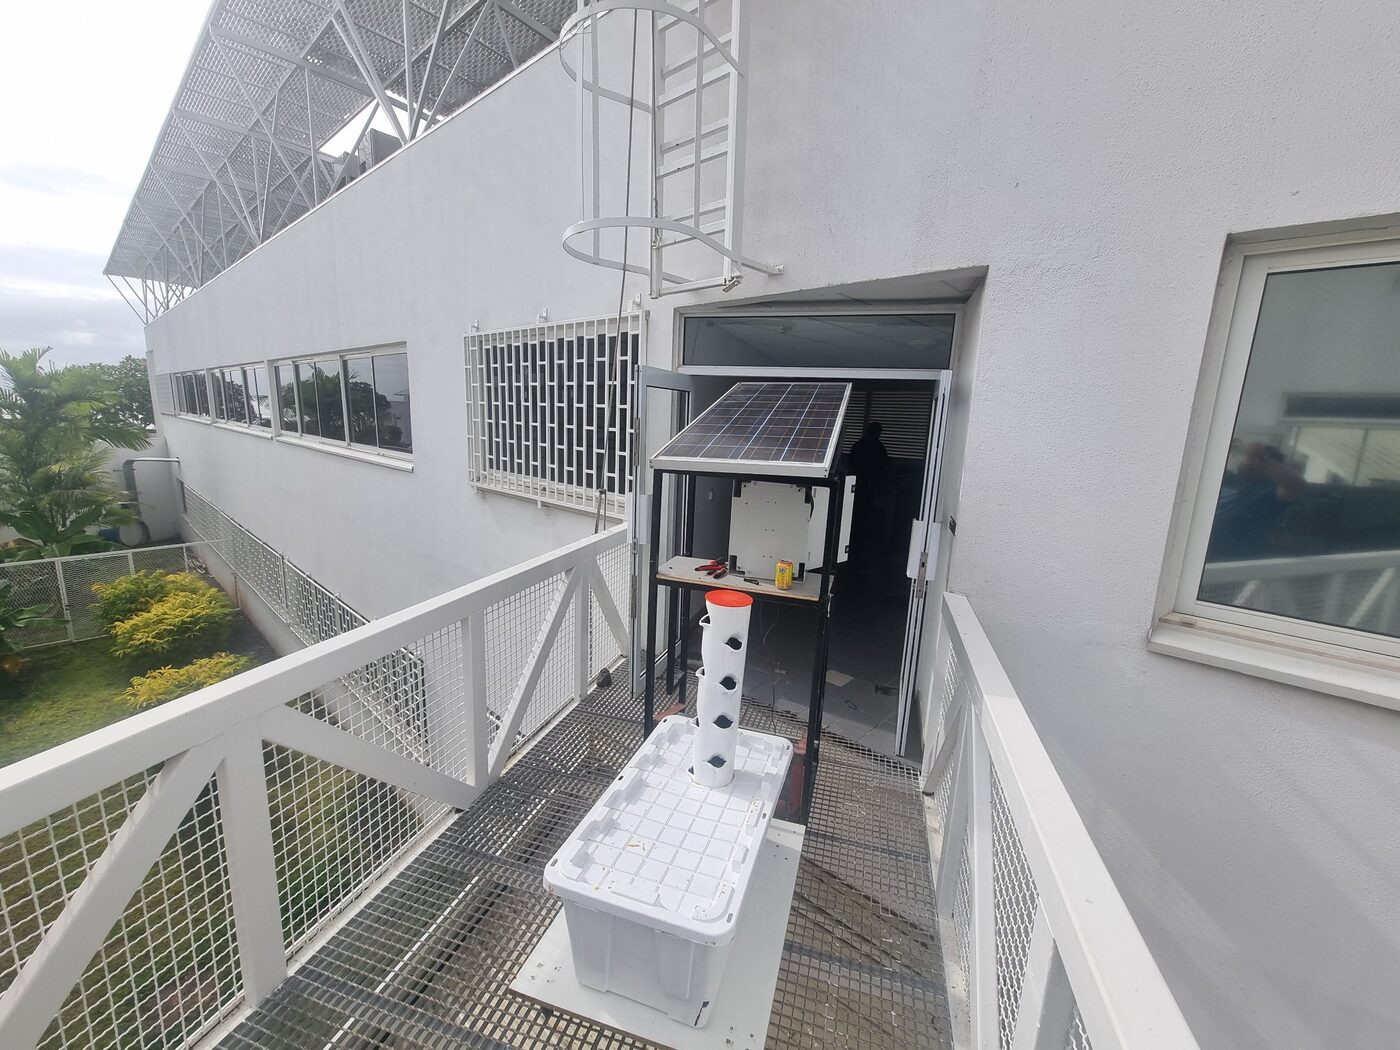
\includegraphics[width=0.9\linewidth]{img/montage/ensemble.jpg}
\caption{Vue d'ensemble : la tour et son bac au premier plan, la structure qui porte le panneau solaire et le plateau de l'armoire derrière.}
\end{figure}

\begin{figure}[H]
\centering
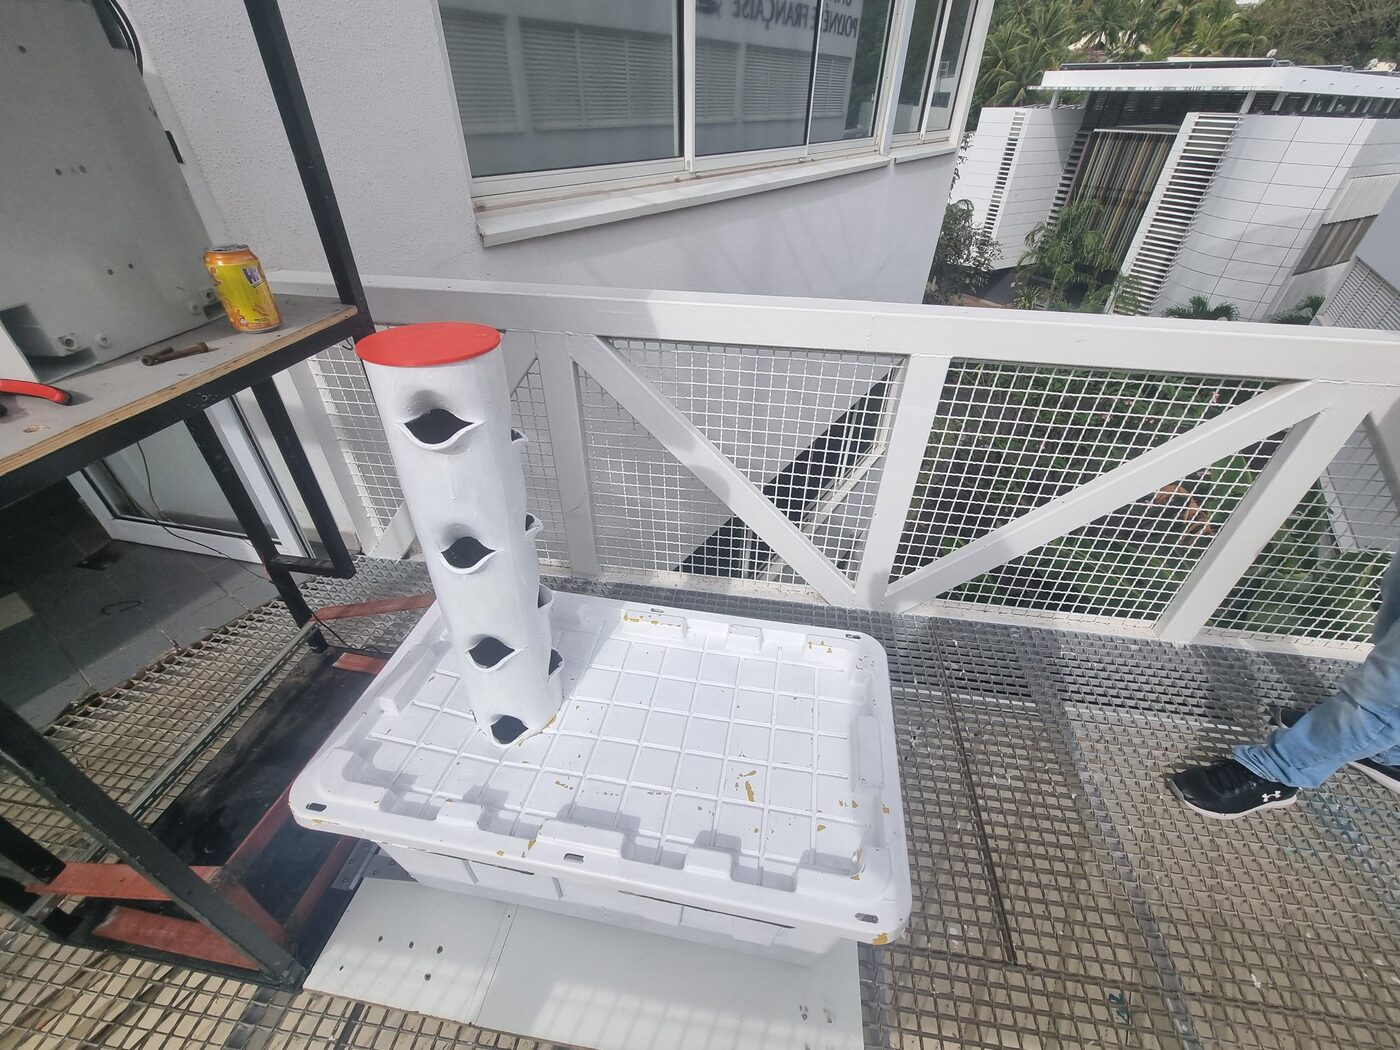
\includegraphics[width=0.78\linewidth]{img/montage/tour.jpg}
\caption{La tour posée sur le couvercle du bac, avec ses trous de plantation.}
\end{figure}

\begin{figure}[H]
\centering
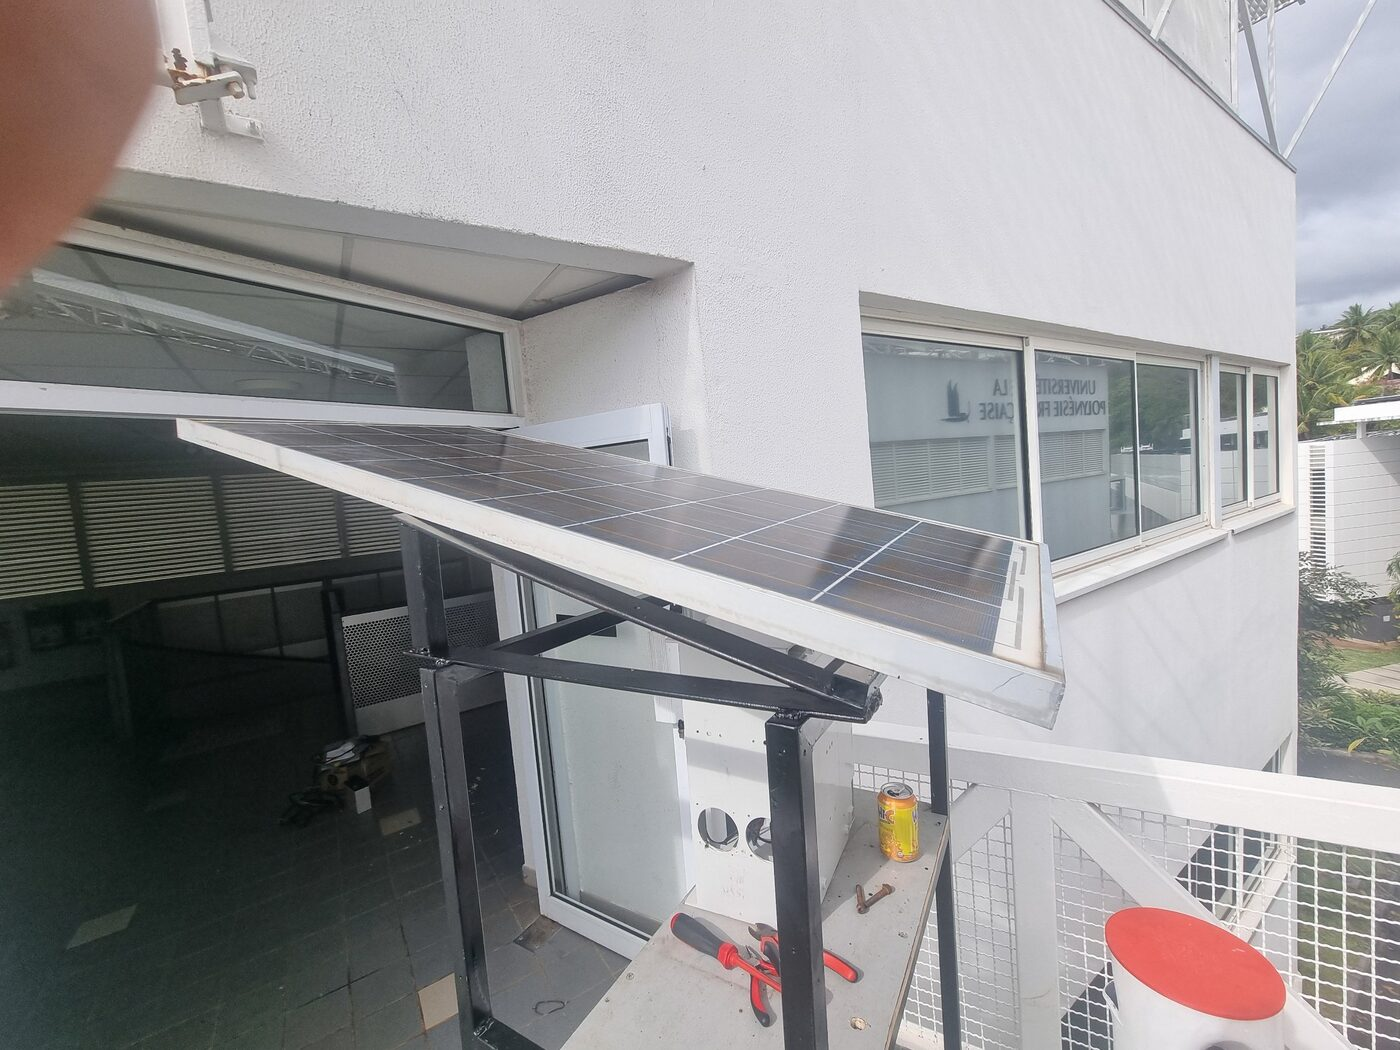
\includegraphics[width=0.9\linewidth]{img/montage/panneau.jpg}
\caption{Le panneau solaire, incliné, sur la structure métallique soudée.}
\end{figure}

\begin{figure}[H]
\centering
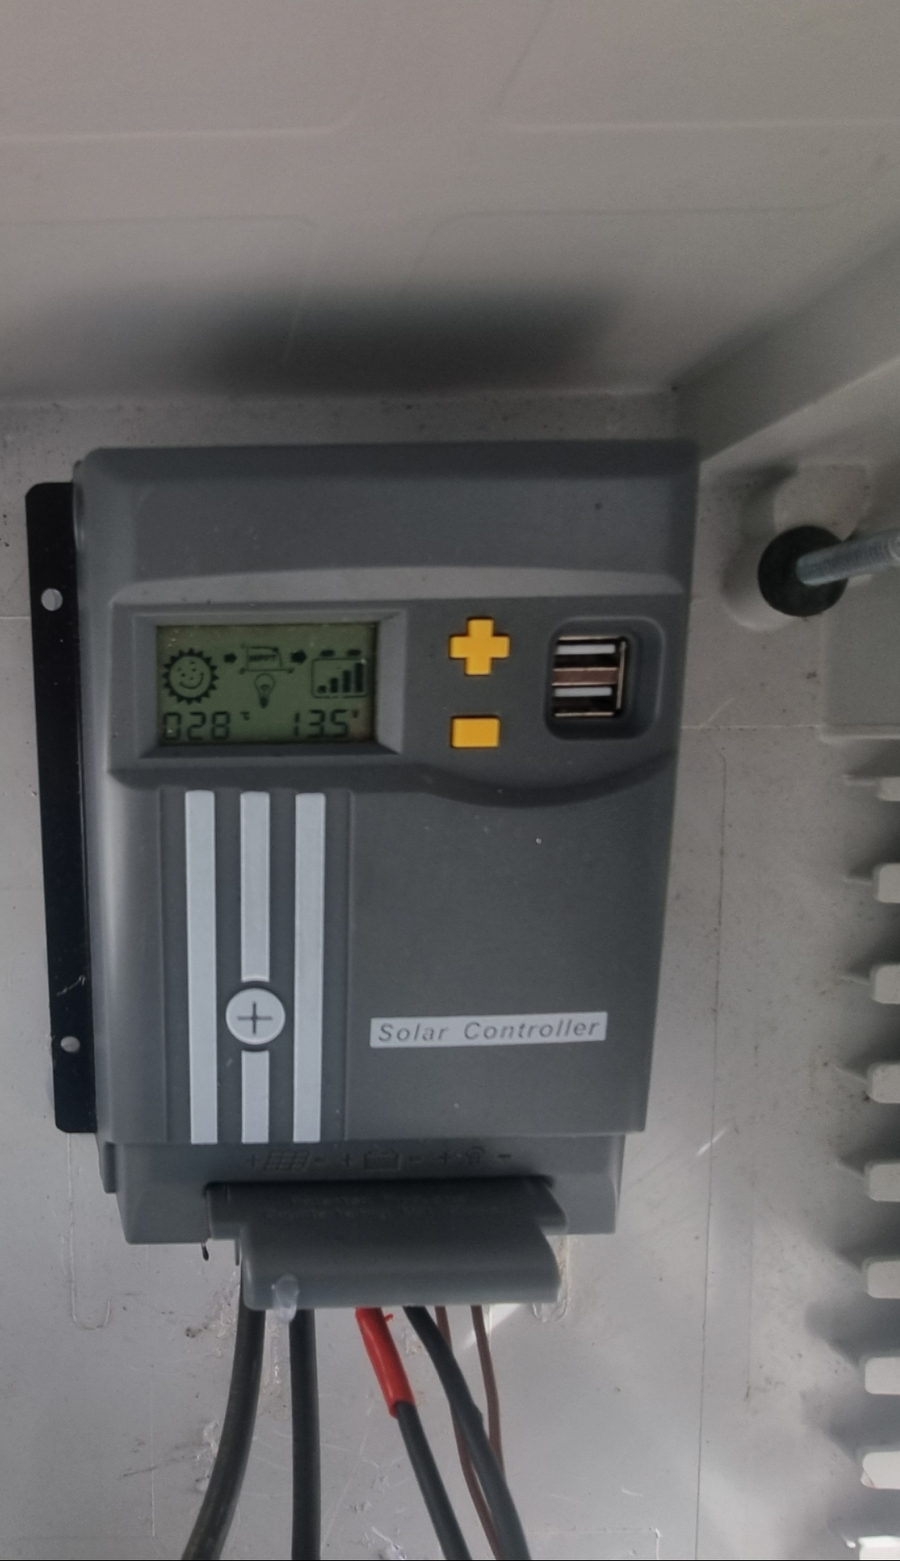
\includegraphics[height=0.32\textheight]{img/montage/regulateur.jpg}
\caption{Le régulateur solaire dans l'armoire, écran allumé (\qty{13,5}{V} au moment de la photo).}
\end{figure}

\textbf{Ce qui reste à faire sur le montage.} Il reste à fixer l'armoire électrique sur le plateau : c'est la suite du travail de Gabriel. De mon côté, je dois modéliser et imprimer le support qui tient la tour dans le bac, puis mesurer le débit réel de la pompe et les pertes de charge réelles du circuit, pour remplacer les valeurs calculées des parties 3 et 4 par des mesures.

\Needspace{8\baselineskip}\subsection{L'état d'avancement}

Le tableau suivant donne l'état d'avancement de chaque fonction de la tour.

\begin{table}[H]
\centering
\scriptsize
\renewcommand{\arraystretch}{1.1}
\begin{tabularx}{\textwidth}{|>{\raggedright\arraybackslash}p{2.6cm}|Y|Y|Y|}
\hline
\textbf{Fonction} & \textbf{Ce qui est fait} & \textbf{Ce qui est vérifié} & \textbf{Ce qui reste} \\
\hline
Circuit d'eau & Débit calculé : \qty{388}{L/h}, \qty{32}{L/h} par plant ; couvercle conçu et imprimé en 3D & Rien mesuré & Mesurer le débit réel, la répartition, la consommation d'eau \\
\hline
Mécanique & Masse du tube, trous, stabilité au vent calculés & Rien mesuré & Peser et mesurer le bac ; lester si bac presque vide \\
\hline
Énergie solaire & Consommation \qty{227}{Wh/j}, production \qty{272}{Wh/j} en juin, batteries, câbles, fusibles calculés & Le 12 novembre : batterie à \qty{13,2}{V}, et le panneau la charge ; rien d'autre mesuré & Lire l'étiquette de la Steco ; mesures M1 à M5 ; limiter le courant de charge \\
\hline
Thermodynamique & Bilan de chaleur du bac, effet du bac blanc, chaleur de la pompe & Rien mesuré & Enregistrer 24 h la température de l'eau et de l'air ; chercher une solution de refroidissement \\
\hline
Sonde EC & Principe, constante $K$ estimée entre \qty{0,97}{cm^{-1}} et \qty{3,04}{cm^{-1}}, formules et schéma & Montée et mesurée dans l'eau le 20 novembre 2026 : \qty{1438}{\micro S\per cm} avec l'étalonnage de départ (partie 9.4) & Étalonner avec deux solutions, en déduire $P$ et $K$ \\
\hline
Sonde de pH & Étalonnage en deux points, formules & Vérifiée le 1\textsuperscript{er} novembre (près d'une demi-heure de mesures) & Étalonner régulièrement ; suivre la dérive \\
\hline
Arduino & ConfigurableFirmata (flash \qty{39,9}{\percent}), coupure des pompes après \qty{30}{s} de silence & Tourne sur la carte depuis le 1\textsuperscript{er} novembre : lecture du pH, de l'air et de l'heure & Essai avec la carte MOSFET\ix{15} et les pompes ; protection locale du niveau à ajouter \\
\hline
Raspberry Pi & Programme de pilotage (\texttt{pilote.py}), serveur, dashboard, accès à distance & Chaîne de mesure vérifiée le 1\textsuperscript{er} novembre ; pilotage testé avec un Arduino simulé & Essai du pilotage sur les vraies pompes, planning de jour et de nuit compris \\
\hline
Plantes & Semis le 27 octobre & Laitues d'environ \qty{5}{cm} au 11 novembre & Repiquage vers le 14 novembre, passage à l'eau nutritive, récolte vers le 16 décembre \\
\hline
Finances & Investissement \qty{101863}{XPF}, coût annuel \qty{12260}{XPF}, retour \qty{2,9}{ans} & Prix indicatifs à confirmer & Relever les vrais prix (engrais, correcteur de pH, laitue au marché) \\
\hline
\end{tabularx}
\caption{État d'avancement de chaque fonction de la tour.}
\end{table}

\Needspace{8\baselineskip}\subsection{Les points ouverts}

Plusieurs hypothèses de ce rapport doivent être remplacées par des mesures. Le régulateur est un SLC-MT2024 alors que l'étude électrique de départ prévoyait un autre modèle (SLC-MPPT2420D) : j'ai recalculé avec la fiche du SLC-MT2024, mais le courant de charge réglable reste à lire dans sa notice. La technologie de la batterie Steco est à lire sur son étiquette, car je l'ai supposée de type AGM comme la Yuasa. Le prix du tube de PVC est un prix équivalent pour un diamètre de \qty{160}{mm}. Les dimensions du bac, les masses, le coefficient d'échange thermique, le débit des doseuses et la hauteur du tuyau de montée sont des hypothèses. Pour la protection de la pompe contre la marche à sec, l'Arduino actuel ne lit pas le niveau d'eau : cette fonction est à ajouter ou à confirmer. Pour la sonde EC, la sonde est maintenant montée et mesure, mais la constante de cellule reste inconnue tant que l'étalonnage à deux solutions n'est pas fait : la valeur affichée aujourd'hui repose sur la constante estimée. Enfin, le tuyau de la tour (flexible de \qty{9}{mm}) limite le débit : il faut mesurer le débit réel.

Un point reste important pour les plantes : d'après le bilan thermique complet (partie 6), l'eau du bac sera vers \qtyrange{26}{27}{\celsius} avec un air à \qty{27}{\celsius} (le premier calcul, plus simple, donnait \qty{28}{\celsius}), au-dessus de la plage idéale de la laitue. C'est un scénario calculé qui repose sur des hypothèses non mesurées (part de la chaleur d'évaporation prélevée dans l'eau, ciel dégagé la moitié du temps) et que l'enregistrement de 24 h doit confirmer. C'est le premier problème que les essais devront résoudre.

\Needspace{8\baselineskip}\subsection{Les prochaines étapes}

D'abord, je modélise et j'imprime le support de la tour dans le bac, puis je mesure le débit réel de la pompe et les pertes de charge réelles. Je repique ensuite les laitues dans la tour vers le 14 novembre, avec de l'eau seule, pour mesurer le débit et la répartition. Ensuite, je passe à l'eau nutritive en suivant le pH et l'EC à la main. La sonde EC étant désormais montée et en service, il me reste à l'étalonner avec les deux solutions. Une fois ces mesures faites, je branche l'Arduino aux pompes pour les premiers essais du pilotage automatique, avec la circulation d'abord, puis les doseuses. Enfin, je remplace les hypothèses par les mesures et je mets à jour ce rapport.

\begin{aretenir}
Le projet est abouti sur le papier : chaque fonction est dimensionnée et démontrée. Il lui manque surtout des mesures sur le vrai matériel. Les trois priorités sont : mesurer la température de l'eau, vérifier la batterie Steco avant de relier les deux batteries, et essayer le programme de l'Arduino sur les pompes.
\end{aretenir}

